\documentclass[french, 9pt,xcolor={table,dvipsnames},t,aspectratio=169,onlytextwidth,mathserif]{beamer}

\usetheme{PSU}

% \setbeamercovered{still covered={\opaqueness<1->{0}},again covered={\opaqueness<1->{40}}}

\usepackage{booktabs}
\usepackage{amsmath}
\usepackage{units}
\usepackage{mathrsfs} 
\usepackage[english,french]{babel}
\usepackage{hyperref}

\newtheorem*{remark}{Remarque} % Création d'un nouvel environnement "Remarque"

% Contenu de la page de garde
\title[Stage ČVUT]{Étude théorique : stations de base du réseau téléphonique français}
\subtitle{Progression du stage}
\author{Paul MÉHAUD, Brendan SÉVELLEC}
\institute{České Vysoké Učení Technické v Praze}
\date{mai - août 2024}

\begin{document}

\begin{frame}
  \titlepage
\end{frame}


\begin{frame}{Déroulé de la présentation}
    \tableofcontents
\end{frame}
\addtocontents{toc}{\protect\setcounter{tocdepth}{1}}

\input{intro}

\section{Semaine du 07/05/24 au 14/05/24}
\insertsectionframe
\subsection{Brendan}
\insertsubsectionframe

{
\smallframetitle
\subsubsection{Affichages}
\begin{frame}{Affichage des données sur une carte}
    \begin{block}{Détail}
        \begin{itemize}
            \item Découverte d'une bibliothèque d'affichage de données géographiques interactive : \texttt{Folium} ;
            \item Affichage des données et colorisation selon plusieurs critères : technologies (2G, 3G, \dots) ou opérateurs (Free, SFR, Bouygues Telecom ou Orange).
        \end{itemize}
    \end{block}

    \begin{alertblock}{Problème}
        Le nombre de données à afficher est très important et rend la visualisation très saccadée.
    \end{alertblock}

    \begin{block}{Solution}
        Afficher seulement une partie des données à la fois selon différent critères de sélection : par opérateurs, technologie ou région.
    \end{block}
\end{frame}



\begin{frame}{}
    \begin{figure}
        \includegraphics[width=0.7\textwidth]{images/France-Opérateurs.png}
        \caption{\label{fig:fr-op}Les opérateurs dans toute la France}
    \end{figure}
\end{frame}

\begin{frame}{}
    \begin{figure}
        \includegraphics[width=0.7\textwidth]{images/France-Technologies.png}
        \caption{\label{fig:fr-tech}Les technologies dans toute la France}
    \end{figure}
\end{frame}

\begin{frame}{}
    \begin{figure}
        \includegraphics[width=0.7\textwidth]{images/Normandie-Opérateurs.png}
        \caption{\label{fig:no-op}Les opérateurs en Normandie}
    \end{figure}
\end{frame}

\begin{frame}{}
    \begin{figure}
        \includegraphics[width=0.7\textwidth]{images/Normandie-Technologies.png}
        \caption{\label{fig:no-tech}Les technologies en Normandie}
    \end{figure}
\end{frame}

\subsubsection{DBScan}
\begin{frame}{Détection des villes}
    Il est très clair que les stations de bases sont très regroupé au sein des villes. Il semble donc qu'il soit possible de détecter si les stations de bases sont en zone rurale ou urbaine à l'aide de la densité de stations de base

    \begin{block}{DBscan (1996)}
        L'algorithme DBscan (Density-Based spatial clustering of applications with noise) est un algorithme qui s'appuie sur la densité estimée des clusters pour effectuer le partitionnement.
    \end{block}
    \begin{block}{Paramètres}
        \begin{itemize}
            \item $\varepsilon$ : dissimilarité maximum entre deux individus ;
            \item $n_{\min}$ : cardinal minimum de chaque classe.
        \end{itemize}
    \end{block}
\end{frame}

\begin{frame}{Théorie : l'algorithme}
    \begin{block}{}
        \begin{enumerate}
            \item Pour chaque point $p_{j}$ :
                \begin{align*}
                    N\left(p_{i}\right) & \gets\left\{ p_{j}, j\in N=\left\{ 1, \dots, n\right\} \mid d(i,j)\leqslant\varepsilon\right\} \\
                    C & \gets\left\{ p_{i}\mid\left|N\left(p_{i}\right)\right|\geqslant n_{\min}\right\} 
                \end{align*}
            \item Construire le graphe de voisinage $G=\left(X, U\right)$, avec $$X=\left\{ p_{i}\mid i\in N\right\} \text{ et } U=\left\{ ij\mid i, j\in N,d(i,j)\leqslant\varepsilon\right\}$$
            \item Trouver les composantes connexes des sommets de $G$ (notées $G_{1}, \dots, G_{p}$) ;
            \item Pour chaque $p_{i}\notin C$ :
                \begin{align*}
                    j^{*} & =\arg\min_{1, \dots, p}\left(d\left(p_{i}, C_{k}\right)\right)\\
                    \text{si } & d\left(p_{i}, C_{j^{*}}\right)\leqslant\varepsilon\text{ alors}\\
                     & C_{j^{*}}\gets C_{j^{*}}\cup\left\{ p_{i}\right\} 
                \end{align*}
        \end{enumerate}
    \end{block}    
\end{frame}

\begin{frame}{}
    \begin{figure}
        \includegraphics[width=0.7\textwidth]{images/France-Villes-Orange_0.03_15.png}
        \caption{\label{fig:fr-vi-or-0.03-15}Les villes détectées en France pour l'opérateur Orange avec $\epsilon=0.03$ et $n_{min}=15$}
    \end{figure}
\end{frame}


\subsubsection{Delaunay et Voronoï}

\begin{frame}{Diagramme de Voronoï}
    \begin{columns}
        \begin{column}{0.6\textwidth}
            \begin{block}{Définition}
                Le diagramme de Voronoï associé à un ensemble de points $(d_i)_{1\leq i \leq n}$ est un pavage de l'espace tel que chaque pavé $P_i$ représente l'ensemble des points plus proches de $d_i$ que de n'importe quel $d_j$ avec $j\neq i$ i.e.
            \end{block}
        \end{column}
            
        \begin{column}{0.4\textwidth}
            \begin{figure}
                \includegraphics[width=0.5\textwidth]{images/Coloured_Voronoi_2D.png}
                \caption{\label{fig:vor-ex}Exemple de diagramme de Voronoï}
            \end{figure}
        \end{column}
    \end{columns}
    
            
\end{frame}

\begin{frame}{Triangulation de Delaunay}
    \begin{columns}
        \begin{column}{0.6\textwidth}
            \begin{block}{Définition}
                La triangulation de Delaunay d'un ensemble $P$ de points du plan est une triangulation $DT(P)$ telle qu'aucun point de $P$ n'est à l'intérieur du cercle circonscrit d'un des triangles de $DT(P)$. Les triangulations de Delaunay maximisent le plus petit angle de l'ensemble des angles des triangles, évitant ainsi les triangles \og allongés \fg{}.
            \end{block}
        \end{column}
            
        \begin{column}{0.4\textwidth}
             \begin{figure}
                \includegraphics[width=0.5\textwidth]{images/Delaunay_circumcircles_vectorial.svg.png}
                \caption{\label{fig:del-ex}Exemple de triangulation de Delaunay}
            \end{figure}
        \end{column}
    \end{columns}
\end{frame}

\begin{frame}{Lien entre les 2}
    \begin{columns}
        \begin{column}{0.6\textwidth}
            \begin{block}{Propriétés}
                \begin{itemize}
                    \item La triangulation de Delaunay d’un ensemble discret $P$ de points est le graphe dual du diagramme de Voronoï associé à $P$;
                    \item Il est donc très facile de passer de l'un à l'autre (en temps polynomial);
                    \item il existe des algorithmes pour trouver une triangulation de Delaunay en $O(n\log(n))$.
                \end{itemize}      
            \end{block} 
        \end{column}
            
        \begin{column}{0.4\textwidth}
            \begin{figure}
                \includegraphics[width=0.5\textwidth]{images/Delaunay_Voronoi.png}
                \caption{\label{fig:del-vor}Lien entre Delaunay et Voronoï}
            \end{figure}
        \end{column}
    \end{columns} 
\end{frame}

\begin{frame}{Retour au problème}
    \begin{block}{Application à notre cas d'étude}
        Nous allons pouvoir utiliser ces notions en définissant :
        \begin{itemize}
            \item les voisins potentiels comme étant les triangles adjacents dans la triangulation de Delaunay
            \item les zones de couverture des antennes comme les pavés associé dans le diagramme de Voronoï
        \end{itemize}
    \end{block}
\end{frame}
}

\subsection{Paul}
\insertsubsectionframe

\begin{frame}{Résumé des épisodes précédents}
    Mon travail, pour la semaine qui vient de s'écouler, s'articule autour de trois axes majeurs :
    \begin{block}{}
        \begin{itemize}
            \item Découverte des données ;
            \item Documentation ;
            \item Reprise du travail de l'année précédente.
        \end{itemize}
    \end{block}
        
\end{frame}

{
\smallframetitle
\begin{frame}{Documentation}
    La majeure partie du travail de la semaine écoulée a consisté à se former aux différents outils de \texttt{Python} afin de pouvoir effectuer sereinement le travail.

    \begin{block}{Outils utilisés}
        \begin{itemize}
            \item \texttt{pandas.DataFrame} : gestion des données ;
            \item \texttt{scipy.spatial.Delaunay} : création de la triangulation de Delaunay ;
            \item \texttt{networkx.Graph} : création de graphes ;
            \item \texttt{matplotlib.pyplot} : affichage des résultats.
        \end{itemize}
    \end{block}
\end{frame}

\begin{frame}{Reprise du travail précédent (1/3)}
    La première tâche consistait à essayer de faire fonctionner le code fourni. Résultat : il ne fonctionne pas\dots
    
    Décision : refaire par moi-même. Cependant, j'ai gardé les idées.
    \begin{block}{Approche pour déterminer les voisins de stations de base}
        \begin{itemize}
            \item Faire une triangulation de Delaunay (liste de voisins potentiels);
            \item Eliminer les voisins distants de plus de $\unit[15]{km}$ ;
            \item Garder le voisin le plus proche dans chaque cadrant autour de chaque station (6 cadrants);
            \item Garder le voisin le plus proche quand deux stations voisines sont séparées par un angle faible.
        \end{itemize}
            
    \end{block}
\end{frame}

\begin{frame}{Reprise du travail précédent (2/3)}
    Ayant refait l'implantation moi-même, j'ai décidé d'utiliser les graphes au lieu de simplement les datasFrames : permettra de faciliter l'application de la théorie des graphes.
    \begin{block}{Apports de cette nouvelle représentation}
        \begin{itemize}
            \item On travail directement sur le graphe de Delaunay ;
            \item Le traitement des voisins est beaucoup plus facile ;
            \item La représentation graphique est plus claire.
        \end{itemize}
    \end{block}
\end{frame}

\begin{frame}{Reprise du travail précédent (3/3) : Résultats}
    Pour l'instant seul les deux premiers critères de filtrage sont fonctionnels. Voici ce que l'on obtient sur le département du Gard :
    \begin{figure}
        \includegraphics[width=0.9\textwidth]{images/comparaison_criteres.png}
        \caption{\label{fig:comp-crit}Evolution de la triangulation de Delaunay en fonction de critères de filtrage}
    \end{figure}
\end{frame}

\begin{frame}{Perspectives d'amélioration et travail à venir}
    \begin{block}{Améliorations}
        \begin{itemize} 
            \item Vérifier que l'algorithme du critère du quadrant donne les bons résultats;
            \item Optimisation dudit algorithme.
        \end{itemize}
    \end{block}

    \begin{block}{Travail à venir}
        \begin{itemize} 
            \item Implanter une version fonctionnelle du critère de l'angle;
            \item Se renseigner sur l'état de l'art de la théorie des graphes.
        \end{itemize}
    \end{block}
\end{frame}
}




\subsection{Brendan}
\insertsubsectionframe
\begin{frame}{Réalisation d'une interface graphique en \texttt{Python}}
    \begin{block}{Contexte}
        \begin{itemize}
            \item Beaucoup de cartes à tracer car beaucoup de paramètres ;
            \item Cartes gourmandes en ressources et pas adaptées à des notebooks \texttt{Python} ;
            \item Réalisation d'une application permettant de facilement tracer ces cartes au sein d'un navigateur web.
        \end{itemize}
    \end{block}
    
\end{frame}

\smallframetitle

\section{Semaine du 14/05/24 au 21/05/24}
\insertsectionframe
\subsection{Le jeu de donnée}
\insertsubsectionframe

\begin{frame}{Le jeu de donnée}
    \begin{block}{Arcep}
        L'autorité de régulation des communications électroniques, des postes et de la distribution de la presse (Arcep) est une autorité administrative indépendante française chargée de réguler les communications électroniques et postales et la distribution de la presse.
    \end{block}

    \begin{block}{Mon Réseau Mobile}
        Mon Réseau Mobile est la plate-forme cartographique regroupant l’ensemble des données géographiques en lien avec les réseaux dits \og mobiles \fg{} (2G, 3G, 4G, 5G) régulés par l’Arcep.
    \end{block}
\end{frame}


\begin{frame}{Arborescence du jeu de données}
    \begin{columns}
        \begin{column}{0.4\textwidth}
            Les fichiers de données sont rangés par trimestre de publication, zone (France métropolitaine/Outre-mer) et département le cas échéant :
        \end{column}
            
        \begin{column}{0.6\textwidth}
            \begin{figure}
                \includegraphics[height=0.55\paperheight]{images/architecture.png}
                \caption{\label{fig:archi}Architecture de la base de donnée}
            \end{figure}
        \end{column}
    \end{columns} 
    
\end{frame}

\begin{frame}{Fréquences de mises à jour}
    \begin{figure}
        \includegraphics[height=0.5\paperheight]{images/frequence.png}
        \caption{\label{fig:freq}Fréquence de publication de mises à jour}
    \end{figure}
\end{frame}


\subsection{Faisons parler les données}
\insertsubsectionframe



\begin{frame}{Comparaison des différents équipements en terme de technologies (1/7)}
    Voici tout d'abord un graphique sur la présence d'une technologie en fonction de l'opérateur (une technologie présente sur un site n'exclue pas la présence d'une autre technologie) :
    \begin{figure}
        \includegraphics[height=0.4\paperheight]{images/barplots/avec_techno.png}
        \caption{\label{fig:av_tech}Nombres de sites équipés d'au moins une technologie}
    \end{figure}
        
\end{frame}

\begin{frame}{Comparaison des différents équipements en terme de technologies (2/7)}
    \begin{table}[!ht]
        \centering
        \footnotesize
        \begin{tabular}{cccccc}
        \hline
            \textbf{Technologie} & \textbf{Bouygues Telecom} & \textbf{Free Mobile} & \textbf{Orange} & \textbf{SFR} & \textbf{Total} \\ \hline
            \textbf{2G} & 4 & 0 & 10 & 20 & 34 \\ 
            \textbf{3G} & 30 & 102 & 65 & 37 & 234 \\ 
            \textbf{4G} & 15 & 15 & 602 & 106 & 738 \\ 
            \textbf{5G} & 0 & 0 & 3 & 0 & 3 \\ 
            \textbf{2-3G} & 66 & 0 & 21 & 80 & 167 \\ 
            \textbf{2-4G} & 12 & 0 & 63 & 67 & 142 \\ 
            \textbf{2-5G} & 0 & 0 & 0 & 0 & 0 \\ 
            \textbf{3-4G} & 3889 & 7225 & 9288 & 4909 & 25311 \\ 
            \textbf{3-5G} & 0 & 0 & 0 & 0 & 0 \\ 
            \textbf{4-5G} & 6 & 0 & 109 & 38 & 153 \\ 
            \textbf{2-3-4G} & 11044 & 0 & 11697 & 9831 & 32572 \\ 
            \textbf{2-3-5G} & 0 & 0 & 1 & 0 & 1 \\ 
            \textbf{2-4-5G} & 0 & 0 & 5 & 10 & 15 \\ 
            \textbf{3-4-5G} & 681 & 18607 & 1638 & 835 & 21761 \\ 
            \textbf{2-3-4-5G} & 10584 & 0 & 7038 & 10085 & 27707 \\ 
            \textbf{Total} & 26331 & 25949 & 30540 & 26018 & 108838 \\ \hline
        \end{tabular}
        \caption{Résumé des données de présence de technologie}
    \end{table}
    
\end{frame}

\begin{frame}{Comparaison des différents équipements en terme de technologies (3/7)}
    Maintenant nous nous intéressons à la fréquence de présence de certaines technologies et pas d'autres :
    \begin{figure}
        \includegraphics[height=0.4\paperheight]{images/barplots/xG.png}
        \caption{\label{fig:xG}Nombres de sites équipés d'une unique technologie}
    \end{figure}
    
\end{frame}

\begin{frame}{Comparaison des différents équipements en terme de technologies (4/7)}
    \begin{figure}
        \includegraphics[height=0.4\paperheight]{images/barplots/2-xG.png}
        \caption{\label{fig:2-xG}Nombres de sites équipés de deux technologies}
    \end{figure}
\end{frame}

\begin{frame}{Comparaison des différents équipements en terme de technologies (5/7)}
    \begin{columns}
        \begin{column}{0.65\textwidth}
            \begin{figure}
                \includegraphics[height=0.4\paperheight]{images/barplots/3-xG.png}
                \caption{\label{fig:3-xG}Nombres de sites équipés de deux technologies (suite)}
            \end{figure}
        \end{column}
            
        \begin{column}{0.35\textwidth}
            \begin{figure}
                \includegraphics[height=0.4\paperheight]{images/barplots/4-5G.png}
                \caption{\label{fig:4-5G}Nombres de sites équipés de deux technologies (suite-bis)}
            \end{figure}
        \end{column}
    \end{columns} 
\end{frame}

\begin{frame}{Comparaison des différents équipements en terme de technologies (6/7)}
    \begin{figure}
        \includegraphics[height=0.4\paperheight]{images/barplots/2-x-yG.png}
        \caption{\label{fig:2-x-yG}Nombres de sites équipés de trois technologies}
    \end{figure}
\end{frame}

\begin{frame}{Comparaison des différents équipements en terme de technologies (7/7)}
    \begin{columns}
        \begin{column}{0.35\textwidth}
            \begin{figure}
                \includegraphics[height=0.4\paperheight]{images/barplots/3-4-5G.png}
                \caption{\label{fig:3-4-5G}Nombres de sites équipés de trois technologies (suite)}
            \end{figure}
        \end{column}
            
        \begin{column}{0.65\textwidth}
            \begin{figure}
                \includegraphics[height=0.4\paperheight]{images/barplots/all-tot.png}
                \caption{\label{fig:all-tot}Nombre de sites équipés de toutes les technologies et total}
            \end{figure}
        \end{column}
    \end{columns} 
\end{frame}

\subsection{Affichage plus détaillé des cartes}
\insertsubsectionframe

\subsubsection{Les stations de base par opérateurs}
\begin{frame}{Les stations de base par opérateur}
    \begin{figure}
        \includegraphics[width=0.9\paperheight]{images/cartes/subplots-providers.png}
        \caption{\label{fig:sp-prov}Les stations de base par opérateurs}
    \end{figure}
\end{frame}


\subsubsection{Les technologies par opérateurs}
\subsubsection{Les technologies par opérateurs}
\begin{frame}{Les stations 2G}
    \begin{figure}
        \includegraphics[width=0.9\paperheight]{images/cartes/site_2g.png}
        \caption{\label{fig:sp-2g}Les stations 2G}
    \end{figure}
\end{frame}

\begin{frame}{Les stations 3G}
    \begin{figure}
        \includegraphics[width=0.9\paperheight]{images/cartes/site_3g.png}
        \caption{\label{fig:sp-3g}Les stations 3G}
    \end{figure}
\end{frame}

\begin{frame}{Les stations 4G}
    \begin{figure}
        \includegraphics[width=0.9\paperheight]{images/cartes/site_4g.png}
        \caption{\label{fig:sp-4g}Les stations 4G}
    \end{figure}
\end{frame}

\begin{frame}{Les stations 5G}
    \begin{figure}
        \includegraphics[width=0.9\paperheight]{images/cartes/site_5g.png}
        \caption{\label{fig:sp-5g}Les stations 5G}
    \end{figure}
\end{frame}


\subsection{Zoom sur la 5g}
\insertsubsectionframe

\begin{frame}{Evolution du nombre de stations 5G en France}
    \begin{figure}
        \includegraphics[height=0.5\paperheight]{images/5g-evolution.png}
        \caption{\label{fig:5g-ev}Evolution du nombre de stations 5G en France}
    \end{figure}
\end{frame}





\input{weeks/21-05_27-05}

\smallframetitle

\section{Semaine du 27/05/24 au 31/05/24}
\insertsectionframe

\subsection{Comparaison des méthodes de détection des villes}
\insertsubsectionframe

\begin{frame}{HDBScan vs DBScan}
    \begin{columns}
        \begin{column}{0.5\textwidth}
            \begin{figure}
                \includegraphics[width=0.4\paperwidth]{images/France-Villes-Orange_0.03_15.png}
                \caption{\label{fig:fr-vi-or-0.03-15-bis}Les villes détectées en France avec DBScan pour l'opérateur Orange avec $\epsilon=0.03$ et $n_{min}=15$}
            \end{figure}
        \end{column}
        \begin{column}{0.5\textwidth}
            \begin{figure}
                \includegraphics[width=0.4\paperwidth]{images/villes_HDBSCAN.png}
                \caption{\label{fig:HDBSCAN-bis}Les villes détectées en France avec HDBScan pour l'opérateur Orange avec \texttt{min\_cluster\_size=5}, \texttt{min\_samples=40}}
            \end{figure}
        \end{column}
    \end{columns}
\end{frame}

\subsection{Amélioration des critères de sélection}
\insertsubsectionframe

\begin{frame}{Prise en compte de la probabilité d'être dans une ville}
    \begin{block}{Concept}
        Chaque station possède une probabilité d'être dans une ville.
        On va donc utiliser ce paramètre afin de moduler l'angle et la distance minimale entre 2 stations.
    \end{block}

    \begin{block}{Choix d'implantation}
        Pour l'instant, on a séparé les stations en 4 catégories, en fonction de la probabilité d'être une ville:
        \begin{itemize}
            \item $p=1$ : \texttt{distance\_max = 1} et \texttt{min\_angle = 45};
            \item $p=0$ : \texttt{distance\_max = 15} et \texttt{min\_angle = 15};
            \item $p\in\left]1 ; 0,6\right[$ : \texttt{distance\_max = 5} et \texttt{min\_angle = 30};
            \item $p\in\left[0,6 ; 0\right[$ : \texttt{distance\_max = 10} et \texttt{min\_angle = 20}.
        \end{itemize}
    \end{block}
    
    \begin{alertblock}{Pistes de travail}
        Il va maintenant falloir effectuer des expérimentations pour trouver les bons paramètres et peut-être essayer de savoir quel paramètre est le plus pertinent.
    \end{alertblock}
\end{frame}

\begin{frame}{Améliorations des cadrants}
    \begin{block}{KNN}
        Dans un premier temps, nous avons décidé de pouvoir chosir le nombre de voisins par cadran que nous souhaitons conserver.
        Cette amélioration ne semble pas très concluante car la méthode devient trop permissive pour $k \geq 2$ (4190 / 4337 voisins conservés).
    \end{block}
    \begin{block}{Optimisation du positionnement des cadrans}
        La position de cadran est choisie en testant un angle $\alpha$ qui est décalage angulaire pour positionner le cadran.
        L'angle alpha choisi est la valeur entre o et 60 degrés qui maximise la distance entre les points et la limite de cadran la plus proche
    \end{block}
\end{frame}

\begin{frame}{Illustration de l'optimisation du positionnement du cadran}
    \begin{columns}
        \begin{column}{0.5\textwidth}
            \begin{figure}
                \includegraphics[height=0.5\paperheight]{images/quadrants_sans_décalage.png}
                \caption{\label{fig:quad_sans_decalage} Quadrants non optimisés}
            \end{figure}
        \end{column}
        \begin{column}{0.5\textwidth}
            \begin{figure}
                \includegraphics[height=0.5\paperheight]{images/quadrants_avec_décalage.png}
                \caption{\label{fig:quad_avec_decalage} Quadrants optimisés}
            \end{figure}
        \end{column}
    \end{columns}
\end{frame}


\smallframetitle

\section{Semaine du 03/06/24 au 06/06/24}
\insertsectionframe

\subsection{Comparaison des résultats de 2 détection de villes}
\insertsubsectionframe

\begin{frame}{Affichage}
    \begin{columns}
        \begin{column}{0.5\textwidth}
            \begin{block}{Affichage des différences}
                Afin de visualiser les différences, nous pouvons tracer les 2 classifications en même temps sur une carte en adoptant ce code couleur :
                \begin{itemize}
                    \item Rouge : station en ville dans les 2 classification;
                    \item Bleu : station en ville dans exactement 1 classification;
                    \item Vert : station en campagne dans les 2 classifications.
                \end{itemize}
            \end{block}
        \end{column}

        \begin{column}{0.5\textwidth}
            \begin{figure}
                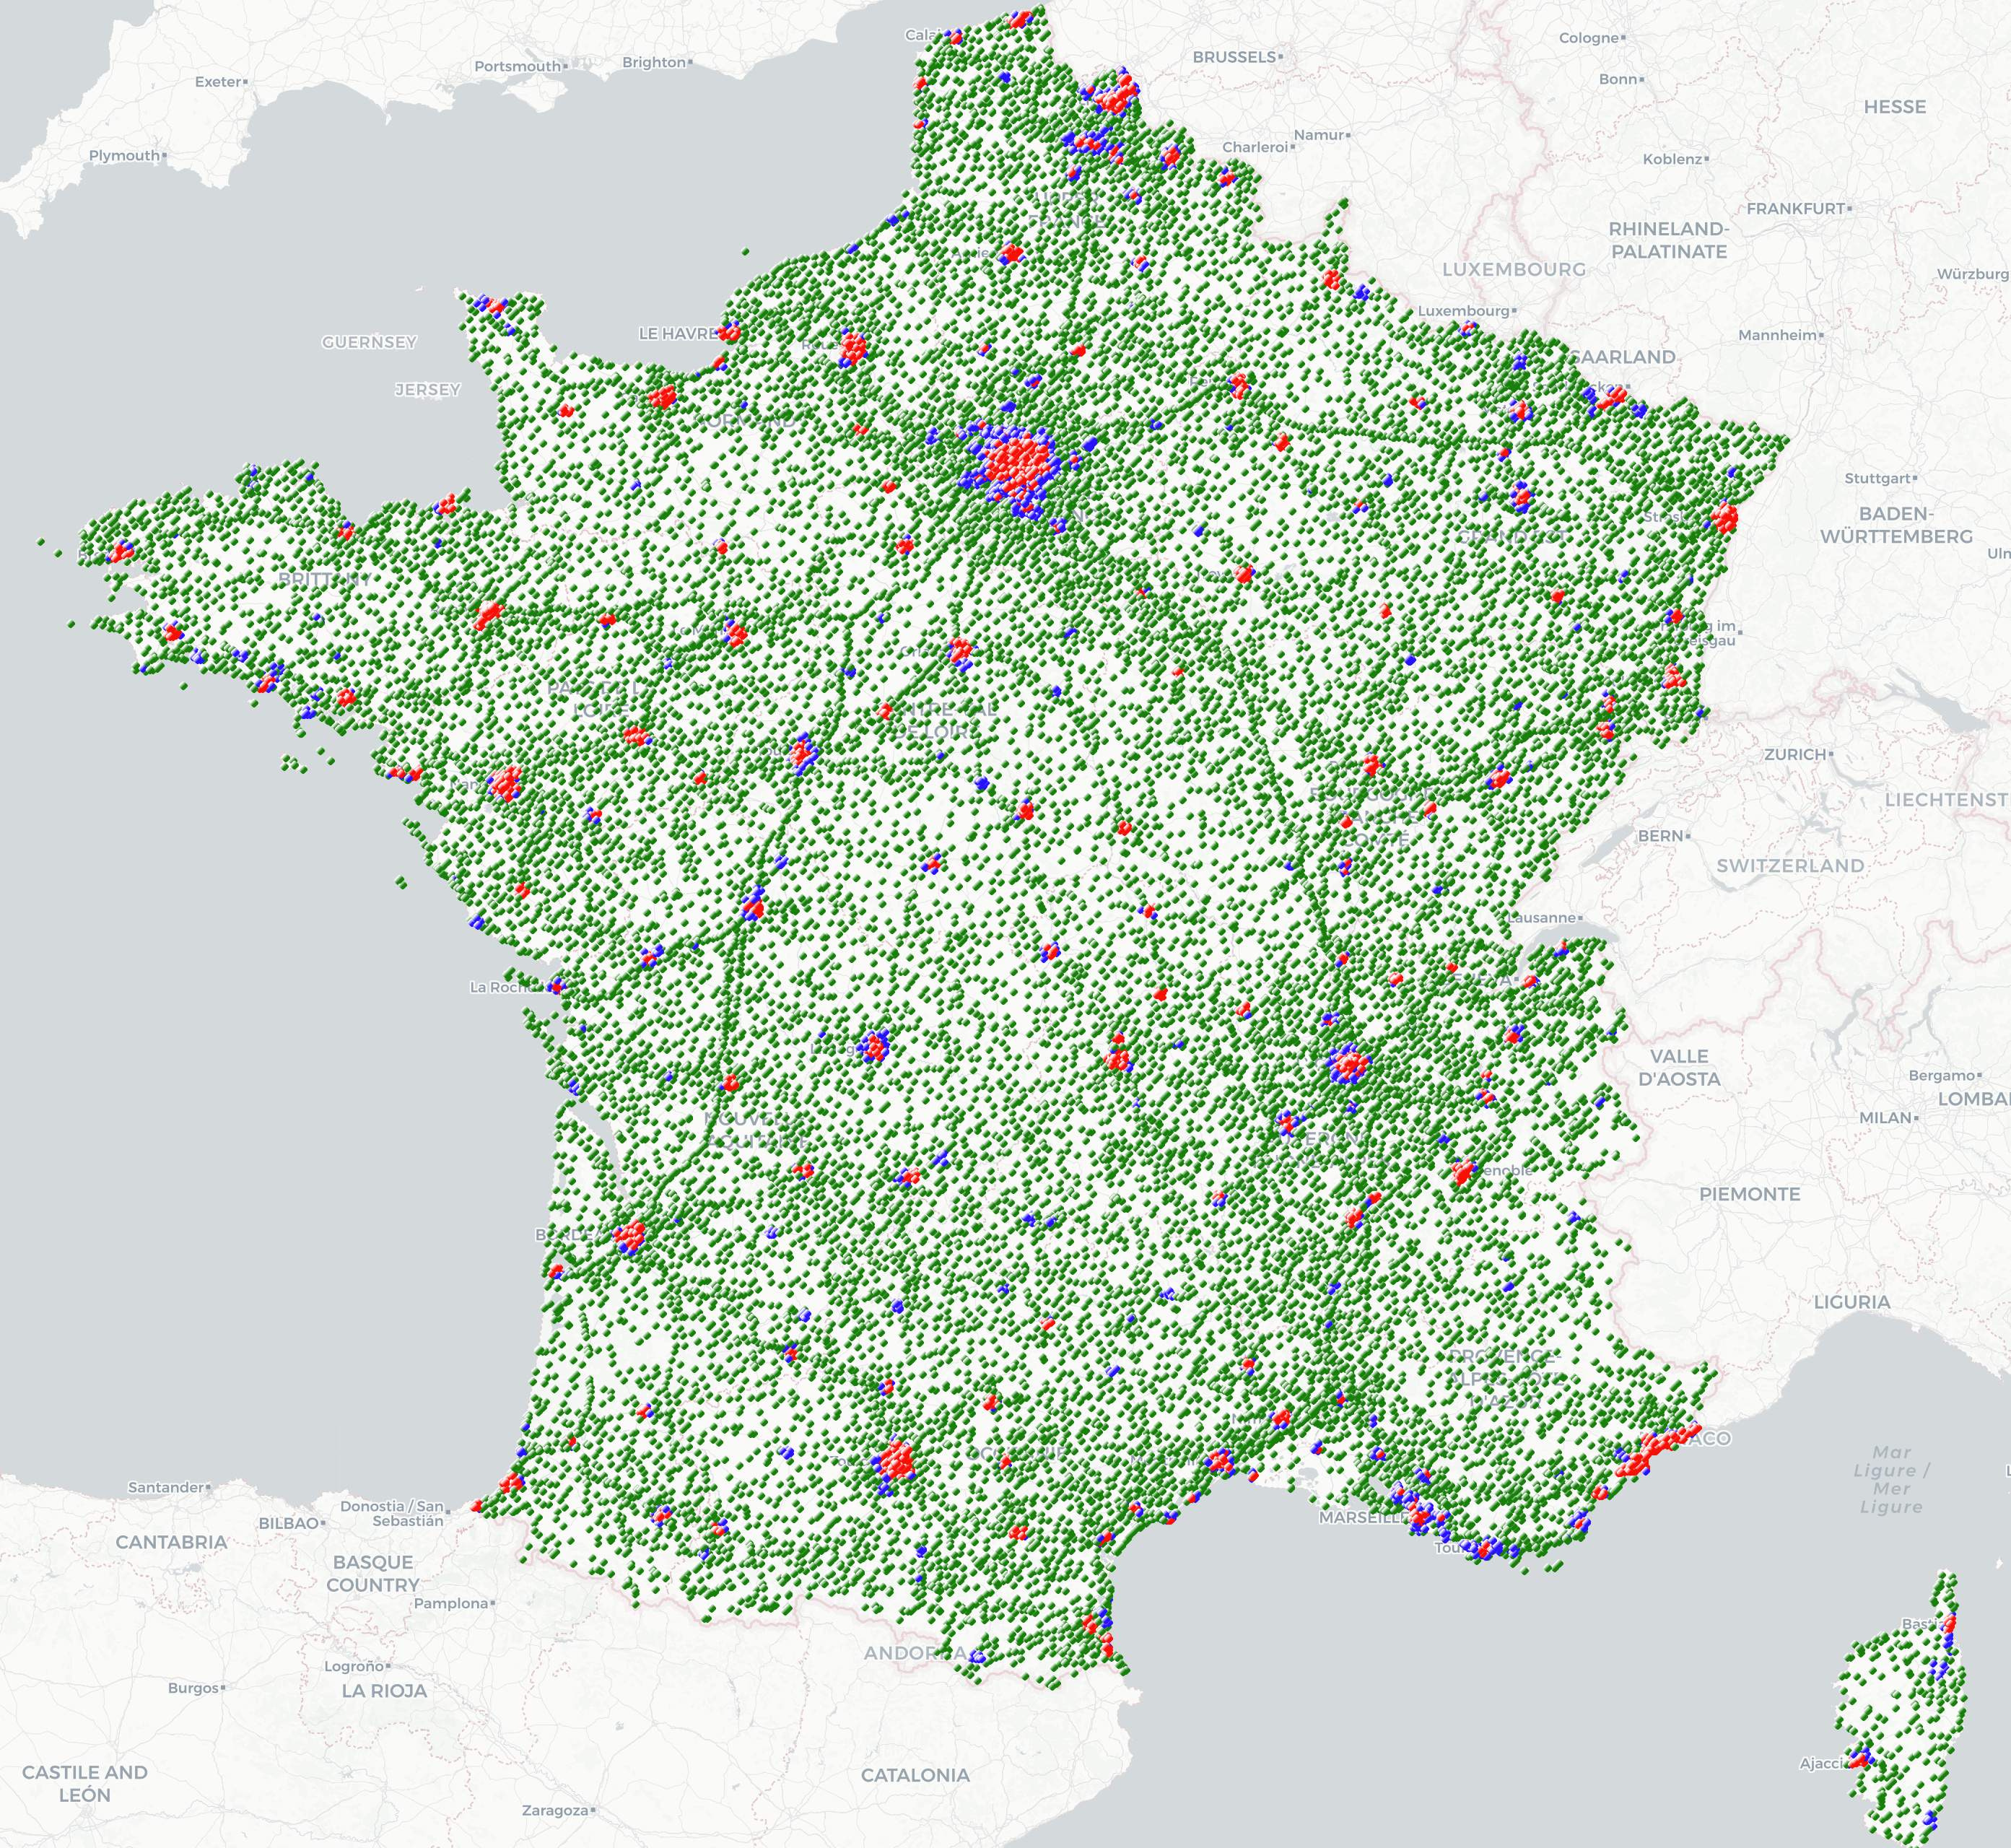
\includegraphics[height=0.5\paperheight]{images/city_comparison.png}
                \caption{\label{fig:city-comparison}Comparaison des résultats de détection de villes : DBScan vs HDBScan}
            \end{figure}
        \end{column}
    \end{columns}
    
    
\end{frame}


\begin{frame}{Indicateurs}
    \begin{block}{Indicateurs de base}
        Nous avons dévéloppé quatre indicateurs de base afin de caractériser la similarité entre deux classifications :
        \begin{itemize}
            \item $a$ : Le pourcentage de station en ville dans les deux classifications;
            \item $b$ : Le pourcentage de station en ville dans la première classifiacation et non la deuxième;
            \item $c$ : Le pourcentage de station en ville dans la deuxième classifiacation et non la première;
            \item $d$ : Le pourcentage de station en campagne dans les deux classifications.
        \end{itemize}
    \end{block}
    \begin{block}{Résultats}
        Sur les classifications présentées dans la slide précédentes, voici les résultats obtenus : 
        \begin{itemize}
            \item $a = 0,688$;
            \item $b = 0,028$;
            \item $c = 0,051$;
            \item $d = 0,232$.
        \end{itemize}
    \end{block}
\end{frame}


\subsection{Nouvelle manière de détecter les villes}
\insertsubsectionframe

\begin{frame}{Changement de cap} 
    \begin{block}{Problèmes rencontrés avec DBScan et HDBScan}
        \begin{itemize}
            \item Méthodes complexes donc peu prévisibles;
            \item Résultats non-satisfaisants quand le méthode est appliquée à seulement une partie de la France.
            \item DBScan est trop binaire, HDBScan est à densité variable donc ne détecte pas toutes les villes de la même façon (problème avec Paris notamment)
            \item Les probabilités de HDBScan ne caractérisent pas exactement la probabilité d'être en ville mais plutôt la certitude avec laquelle on peut rattacher un point à son cluster.
        \end{itemize}
    \end{block}

    \begin{block}{Réflexion sur une méthode plus simple}
        Nous souhaitions savoir quelle station se trouvait en ville, car on sait qu'en ville, les stations sont plus proches les unes des autres, donc les rayons de couverture plus courts.
        Cependant, il n'est pas nécessaire de detecter les villes pour cela, nous pouvons simplement regarder la distance moyenne aux $k$ plus proches voisins.
    \end{block}

\end{frame}

\begin{frame}{Méthodologie}
    \begin{block}{Nouvelle méthode}
        Au lieu d'utiliser une méthode de clustering, nous allons utiliser quelque chose de plus simple.
        On classifie chaque station selon la distance moyenne aux $3$ plus proches voisins. %2 c'est pas assez pour avoir quelquechose de palapable, 4 augmente trop la distance.
        Soit $d$ cette distance, on regroupe les stations de la manière suivante:
        \begin{itemize}
            \item $d\in\left]0, 1\right]$ : centre ville dense;
            \item $d\in\left]1, 2\right]$ : couronne périhurbaine;
            \item $d\in\left]2, 5\right]$ : campagne;
            \item $d\in\left]5, 10\right]$ : campagne profonde;
            \item $d\in\left]10, \infty\right[$ : trou paumé ou valeur aberrante.
        \end{itemize}
    \end{block}
\end{frame}

\begin{frame}{Méthodologie : choix techniques}
    \begin{block}{Calcul des plus proches voisins}
        Nous utilisons la bibliothèque \emph{sklearn.neighbors.NearestNeighbors}\footnotemark.
    \end{block}

    \begin{block}{Choix du nombre de voisins}
        Après plusieurs expérimentations, nous avons choisi de conserver $3$ voisins dans notre calcul.
        En effet, un chiffre inférieur à $2$ serait aberrant car ce ne serait pas une vraie moyenne (ici on cherche plus une mesure de la densité de stations).
        De plus, un chiffre supérieur à $4$ prendrait en compte des stations trop éloignées, ce qui serait aberrant.
    \end{block}
    
    \begin{block}{Métrique}
        Nous avons décidé de partir de la projection de Lambert 93 (qui est déjà présente dans nos données) pour calculer cette distance.
        L'avantage est le gain de temps (environ 30 fois plus rapide), sans perte de performance, par rapport à la conversion en $\unit{km}$ depuis les coordonnées Longitude, Latitude.
    \end{block}

    \footnotetext{\url{https://scikit-learn.org/stable/modules/generated/sklearn.neighbors.NearestNeighbors.html}}
\end{frame}

\begin{frame}{Mise à jour des critères}
    \begin{columns}
        \begin{column}{0.4\paperwidth}
            \begin{block}{Angle}
                Voici les différents paliers que nous appliquons :
                \begin{itemize}
                    \item $d\in\left]0, 1\right]$ : $\text{angle\_min}=40^\circ$;
                    \item $d\in\left]1, 2\right]$ : $\text{angle\_min}=30^\circ$;
                    \item $d\in\left]2, 5\right]$ : $\text{angle\_min}=25^\circ$;
                    \item $d\in\left]5, 10\right]$ : $\text{angle\_min}=15^\circ$;
                    \item $d\in\left]10, \infty\right[$ : $\text{angle\_min}=10^\circ$.
                \end{itemize}
            \end{block}
        \end{column}
        \begin{column}{0.4\paperwidth}
            \begin{block}{Distance}
                Voici les différents paliers que nous appliquons :
                \begin{itemize}
                    \item $d\in\left]0, 1\right]$ : $\text{distance\_max}=\unit[2]{km}$;
                    \item $d\in\left]1, 2\right]$ : $\text{distance\_max}=\unit[5]{km}$;
                    \item $d\in\left]2, 5\right]$ : $\text{distance\_max}=\unit[10]{km}$;
                    \item $d\in\left]5, 10\right]$ : $\text{distance\_max}=\unit[15]{km}$;
                    \item $d\in\left]10, \infty\right[$ : $\text{distance\_max}=\unit[15]{km}$.
                \end{itemize}
            \end{block}
        \end{column}
    \end{columns}
\end{frame}

\smallframetitle

\section{Semaine du 10/06/24 au 14/06/24}
\insertsectionframe

\smallframetitle

\section{From 17/06/24 to 21/06/24}
\insertsectionframe

\subsection{Road detection method - in progress}
\insertsubsectionframe

\begin{frame}{Methodology}
    We have seen that one classification with either DBScan or HDBScan isn't enough. So, why not combining them.
    \begin{block}{The base idea}
        We will combine the clusters of DBScan, HDBScan and OPTICS (another density base clustering method) to try to find roads.
    \end{block}

    \begin{block}{One problem}
        We are now able to detect road/railways but the problem is that there is still little clusters that are useless.
    \end{block}
\end{frame}

\begin{frame}{DBScan clustering}
    \begin{figure}
        \includegraphics[height=0.6\paperheight]{images/cartes/road_detection/dbs.png}
        \caption{DBScan clustering}
    \end{figure}
\end{frame}

\begin{frame}{HDBScan clustering}
    \begin{figure}
        \includegraphics[height=0.6\paperheight]{images/cartes/road_detection/hdb.png}
        \caption{HDBScan clustering}
    \end{figure}
\end{frame}

\begin{frame}{OPTICS clustering}
    \begin{figure}
        \includegraphics[height=0.6\paperheight]{images/cartes/road_detection/opt.png}
        \caption{OPTICS clustering}
    \end{figure}
\end{frame}

\begin{frame}{Result}
    \begin{figure}
        \includegraphics[height=0.6\paperheight]{images/cartes/road_detection/res.png}
        \caption{Road detection}
    \end{figure}
\end{frame}

\subsection{More details and problems}
\insertsubsectionframe

\begin{frame}{Detailed clusters detected}
    \begin{figure}
        \includegraphics[height=0.6\paperheight]{images/clusters_road_detection.html.png}
        \caption{Detailed clusters detected in coutryside by each method}
    \end{figure}
\end{frame}

\begin{frame}{Problems and ideas}
    \begin{block}{Problems}
        \begin{itemize}
            \item A lot of little citys detected : not only roads ;
            \item The areas around big citys are a mess ;
            \item HDBScan has only one cluster.
        \end{itemize}
    \end{block}

    \begin{block}{Ideas}
        \begin{itemize}
            \item Refine the parameters of each method ;
            \item Use linear regressions to detect parts of roads and maybe help propagate them.
        \end{itemize}
    \end{block}
\end{frame}

\subsection{Modification of criteria}
\insertsubsectionframe

\begin{frame}{Altair AI Studio Software Review}
    Objective is to evaluate Altair AI Studio for their potential to enhance our research on classifying the terrain of mobile base stations.
    Available at: \url{https://altair.com/altair-ai-studio}
    \begin{block}{Altair AI Studio}
        This is a platform designed for data analysis and machine learning model building. Possible benefits for us:
        \begin{itemize}
            \item Simplifies data integration and visualization of base station and land cover data.
            \item Supports clustering and classification algorithms.
            \item Support for various machine learning algorithms.
            \item Enables effective result visualization (graphs) for enhanced analysis.
        \end{itemize}
    \end{block}
    \begin{columns}
        \begin{column}{0.4\paperwidth}
            \begin{block}{Key Features:}
                \begin{itemize}
                    \item Integration with various data sources.
                    \item Interactive model creation and testing.
                    \item Support for various machine learning algorithms.
                    \item User-friendly interface for data analysis and visualization.
                \end{itemize}
            \end{block}
        \end{column}
        \begin{column}{0.4\paperwidth}
            \begin{block}{Users:}
                \begin{itemize}
                    \item Data researchers
                    \item Analysts
                    \item Machine learning developers
                \end{itemize}
            \end{block}
        \end{column}
    \end{columns}
\end{frame}

\begin{frame}{Example of Usage in Altair AI Studio}
    \begin{figure}
        \includegraphics[height=0.6\paperheight]{images/Altair/Altair_proc_exmpl.png}
        \caption{How 3-NN method works}
    \end{figure}
\end{frame}


\smallframetitle

\subsection{Analysis of Frequency Data for Mobile Operators in France}
\insertsubsectionframe

\begin{frame}{France spectrum - mobile network frequency plan}
    We have detailed data on the frequency spectrums used by mobile operators in France. This data allows us to understand the specific frequencies at which each base station operates.
    \begin{block}{Frequency Bands:}
        \begin{itemize}
            \item The primary frequency bands used for 4G LTE in France include 700 MHz, 800 MHz, 1800 MHz, 2100 MHz, and 2600 MHz.
            Each frequency band has its own characteristics in terms of range, penetration, and data capacity.
        \end{itemize}
    \end{block}
    \begin{figure}
        \includegraphics[height=0.4\paperheight]{images/Altair/Or_spectrum.png}
        \caption{Orange Mobile network frequency plan}
    \end{figure}
\end{frame}

\begin{frame}{Analysis of Frequency Data for Orange}
    \begin{figure}
        \includegraphics[height=0.6\paperheight]{images/Altair/Or_4g_freq_compar.png}
        \caption{Count of antennas operating at each frequency band}
    \end{figure}
\end{frame}

\begin{frame}{Analysis of Frequency Data}
    \begin{block}{Characteristics of each band}
        \begin{itemize}
            \item 700 MHz and 800 MHz: Long-range, good building penetration.
            \item 1800 MHz and 2100 MHz: Balanced range and capacity.
            \item 2600 MHz: Short-range, high capacity.
        \end{itemize}
    \end{block}

    \begin{block}{Methodology for Coverage Calculation}
        \begin{itemize}
            To estimate the coverage zones of mobile base stations using only frequency data, we can implement the following approach. 
            
            We can apply standard radio propagation models such as the Hata Model for urban areas and the Cost-231 for suburban and rural areas. These models allow us to estimate coverage zones based on the operating frequency of each base station. Despite lacking specific data on transmission power, antenna gain, path loss, and receiver sensitivity, these propagation models provide a generalized prediction of signal coverage areas by leveraging established empirical data and frequency characteristics. This methodology can enable us to approximate the coverage zones for each frequency band.
        \end{itemize}
    \end{block}
\end{frame}

\begin{frame}
    \frametitle{LTE RF Link Budgeting Model}
    \begin{itemize}
        \item The link budget calculations are needed for the calculation of cellular coverage parameters.
        \item A link budget takes into consideration all the losses and gains involved in equipment (e.g., BTS), end-terminals (e.g., mobile devices), and communication medium (e.g., free space).
        \item The results obtained indicate the maximum allowable propagation loss (MAPL). The formulae used in the link budget calculations are expressed below:
    \end{itemize}
    \begin{block}{Link budget calculations}
        \begin{align}
            EIRP_{Tx} &= P_{Tx} + G_{Tx} - L_b \\
            EIRP_{Tx} &= NB_{noise} + Th_{noise} + SINR \\
            MAPL &= EIRP_{Tx} + R_{SENS} - IM - L_{cable} + G_{Rx} - M + G_{soft}
        \end{align}
    \end{block}
    \textbf{Note:} We do not have exact data for our base stations, but we can make reasonable assumptions based on industry standards.
    \end{frame}

\begin{frame}{Reference Research Findings}
    We have referenced research that provides input parameters for radio propagation models and cell-range calculation results.
    \begin{block}{Input parameters for radio propagation model}
        \begin{itemize}
            \item Carrier Frequencys (MHz): 700, 800, 1800, and 2100 MHz.
            \item Base Station Height (hb): Typically around 30 meters.
            \item Mobile Station Height (hm): Generally around 1.5 meters.
        \end{itemize}
    \end{block}
    \begin{figure}
        \includegraphics[height=0.35\paperheight]{images/Altair/cell_range_calc_res.png}
        \caption{Cell-range calculation results}
    \end{figure}
\end{frame}

\begin{frame}{Frequency Reuse Mode Challenges}
    \begin{columns}
        \begin{column}{0.55\textwidth}
            \begin{block}{Challenges with Unknown Frequency Reuse Mode}
                    \begin{itemize}
                        \item Each cell in a mobile network can be divided into sectors, each served by a different frequency.
                        \item The reuse of frequencies in different cells is essential to maximize the efficient use of the available spectrum.
                        \item Frequency reuse mode determines how frequencies are allocated across cells and sectors to minimize interference.
                        \item We lack detailed information on the specific frequency reuse mode utilized for each sector of our base stations.
                        \item Assumptions about uniform frequency reuse may not reflect the actual, varied configurations used in practice.
                    \end{itemize}
            \end{block}
        \end{column}
        \begin{column}{0.6\textwidth}
            \begin{figure}
                \includegraphics[height=0.4\paperheight]{images/Altair/Sectorization.png}
                \caption{\label{fig:ill_HDBScan_4} Sectorization}
            \end{figure}
        \end{column}
    \end{columns}
\end{frame}

\end{document}
